\chapter{Measuring the distance to a galaxy using globular clusters}

%todo add lab activity to measure differential light intensity at different distances from light bulbs
%todo clarify that M5 (rather than Sun) should be used to compare to M87 cluster
%todo describe M classification system, that they can represent different kinds of things

%In this lab, you will measure the distance to the Virgo galaxy, which we will use for next week’s laboratory as the first rung in our distance ladder measuring the distance to other galaxies.

In this lab, we will use a globular cluster in the Milky Way called M5 (see Figure~\ref{gc:fig:m5}) as the first step of our distance
ladder to other galaxies. By comparing this globular cluster to another in a nearby galaxy
called M87 in the Virgo cluster, we will estimate its distance, adding another rung to our
distance ladder. Ideally, we should compare many globular clusters in the Milky Way to
M87, here we will use just one cluster, which is enough to demonstrate the principle.

\begin{figure}
	\centering
	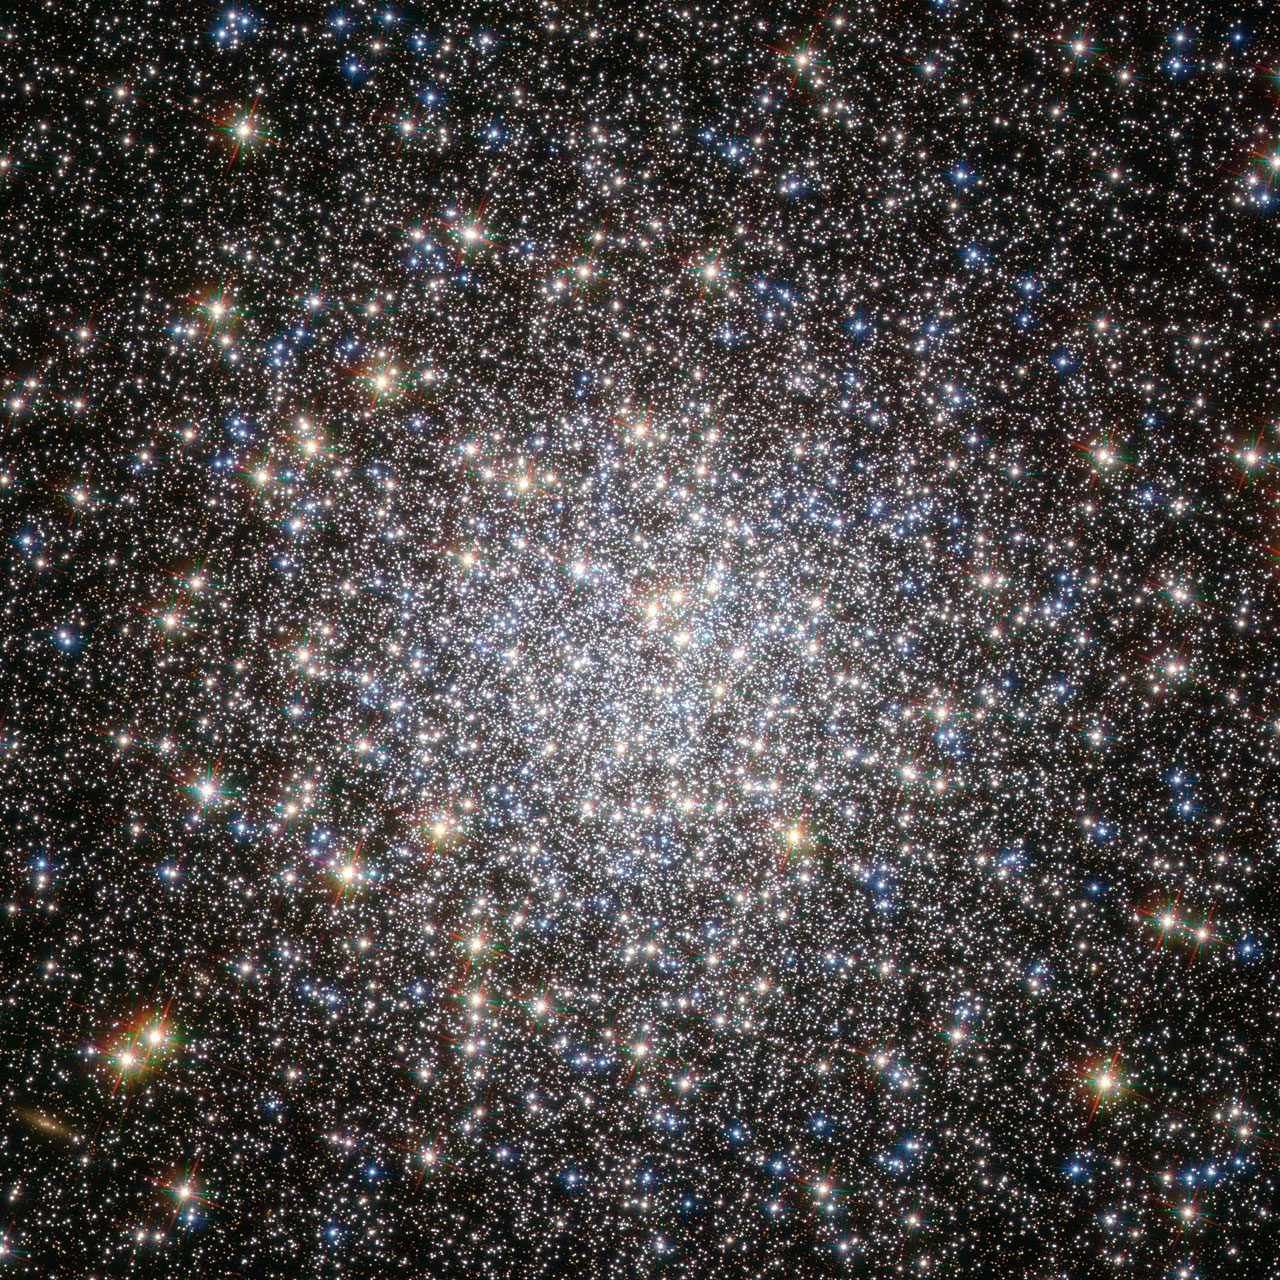
\includegraphics[width=0.7\textwidth]{globular-cluster/potw1118a}
	\caption{Messier 5 (M5) is a globular cluster (a gravitationally bound collection
		of stars) of more than 100,000 stars in the Milky Way Galaxy. Located at Right
		Ascension (RA) = 229.640\textdegree, and Declination (Dec) = 2.075\textdegree.
		The above
		image is 2.85 arcmin on a side, or about 1/20th of a degree.
		Image source: ESA/Hubble \& NASA, \url{http://www.spacetelescope.org/images/potw1118a/}}\label{gc:fig:m5}
\end{figure}

If two identical lightbulbs are placed with one close to you and another farther away, the more distant one will appear dimmer. This is because the light from a spherical emitting source spreads out over a spherical shell that gets larger as the light gets more distant from the source. So if sources 1 and 2 have the same luminosity, then their distances $d$ and apparent brightness
$b$ are related by
\begin{equation}
\frac{b_1}{b_2} = \left( \frac{d_2}{d_1} \right)^2 \,.
\end{equation}
Since the numbers we will extract from the images are either in brightness or magnitudes,
it is convenient to re-cast this relation in terms of magnitudes. Magnitudes $m_1$ and $m_2$ are
related to brightness $b_1$ and $b_2$ by
\begin{equation}
m_2 - m_1 = 2.5 \log \left[ \left( \frac{b_1}{b_2} \right)^2 \right] \,.
\end{equation}
Combining the two equations, we get
\begin{equation}\label{gc:eq:m-d}
 \log(d_1/d_2) = 0.2 (m_1-m_2) \,.
\end{equation}
This says that once we have measured magnitudes $m_1$ and $m_2$ for two sources, then we can
derive the ratio of their distances from us, \textit{as long as they have the same luminosity}.

\section{Road Map}

To keep track of the steps in this lab, we will fill in Table~\ref{gc:tab:mag}. In this table, the entry for the magnitude of M5 refers to the sum of all of its stars. In
principle, we could measure this ourselves with the roof-top telescope, but for this lab we take
a value from a catalog of such data. The SDSS data cannot be used because the stars
are too crowded together for an accurate measurement.

\begin{table}
	\centering
	\begin{tabular}{l|c|c}
		\toprule
		\textbf{Object} & \textbf{Magnitude} & \textbf{Distance (AU)} \\ \midrule
		Sun & -26.89 & 1 \\\midrule
		Sun-like stars in M5 &  & \\\midrule
		M5 itself & 5.65 & \\\midrule
		M87 globular clusters & &
		\\ \bottomrule
	\end{tabular}
	\caption{Table of magnitude and distance.}\label{gc:tab:mag}
\end{table}

The first step is to make a \textit{color-magnitude diagram} for the stars in M5 to find a star that
has similar to the Sun; we assume that such a star has the same luminosity as the Sun. The
magnitude of the star (specifically its $r$-band magnitude) gets entered into the above table,
and you derive the distance to M5.

The second step is to identify faint things surrounding the galaxy M87 that are likely to be
globular clusters associated with it, and get their magnitudes (again the $r$-band magnitude)
from the database. Some value that properly represents the ensemble gets entered into the
above table and you derive the distance to M87 by comparing the magnitudes of M5 and M87.

\textit{To summarize:} the distance to the Virgo cluster depends on two assumptions: 1) stars
with Sun-like colors in the globular cluster M5 have the same luminosity of the Sun. 2)
Globular clusters like M5 in the Milky Way have luminosities that are comparable to
the globular clusters in M87. Neither of these assumptions is necessarily well justified based on information available to you, but there are checks that reassure us that the assumptions
are good enough for at least a first estimate of distance.

\section{Analyzing the M5 globular cluster}

First you'll retrieve from an online database the magnitude of stars in the region of sky where M5 is. In the window at \url{http://skyserver.sdss.org/dr13/en/tools/search/sql.aspx}, enter the following query:

\begin{verbatim}
SELECT TOP 200
   objid,ra,dec,u,g,r,i,z
FROM Star
WHERE
   r BETWEEN 10 AND 23
   AND ra between 229.50 and 229.78
   AND dec between 2.2 and 2.3
\end{verbatim}

\subsection{Questions and results for your report}

\begin{steps}
	\item From the data above, create a .csv file, rename it M5.csv. Read it into
	a spreadsheet, and make columns for the colors $g - r$, $r - i$, and $g - i$. The Sun has
	colors $g - r = 0.44$, $r - i = 0.11$, and $g - i = 0.55$. Plot the $r$ magnitude vs. one of the colors (e.g.
	$g - r$), and reverse the $r$ magnitude axis, since lower magnitudes represent brighter objects. On this color-magnitude diagram, identify
	the \textit{main sequence} of stars. This plot is called a color-magnitude diagram, which is similar to an H-R diagram as seen in Figure~\ref{gc:fig:hr}.
\end{steps}

\begin{figure}
	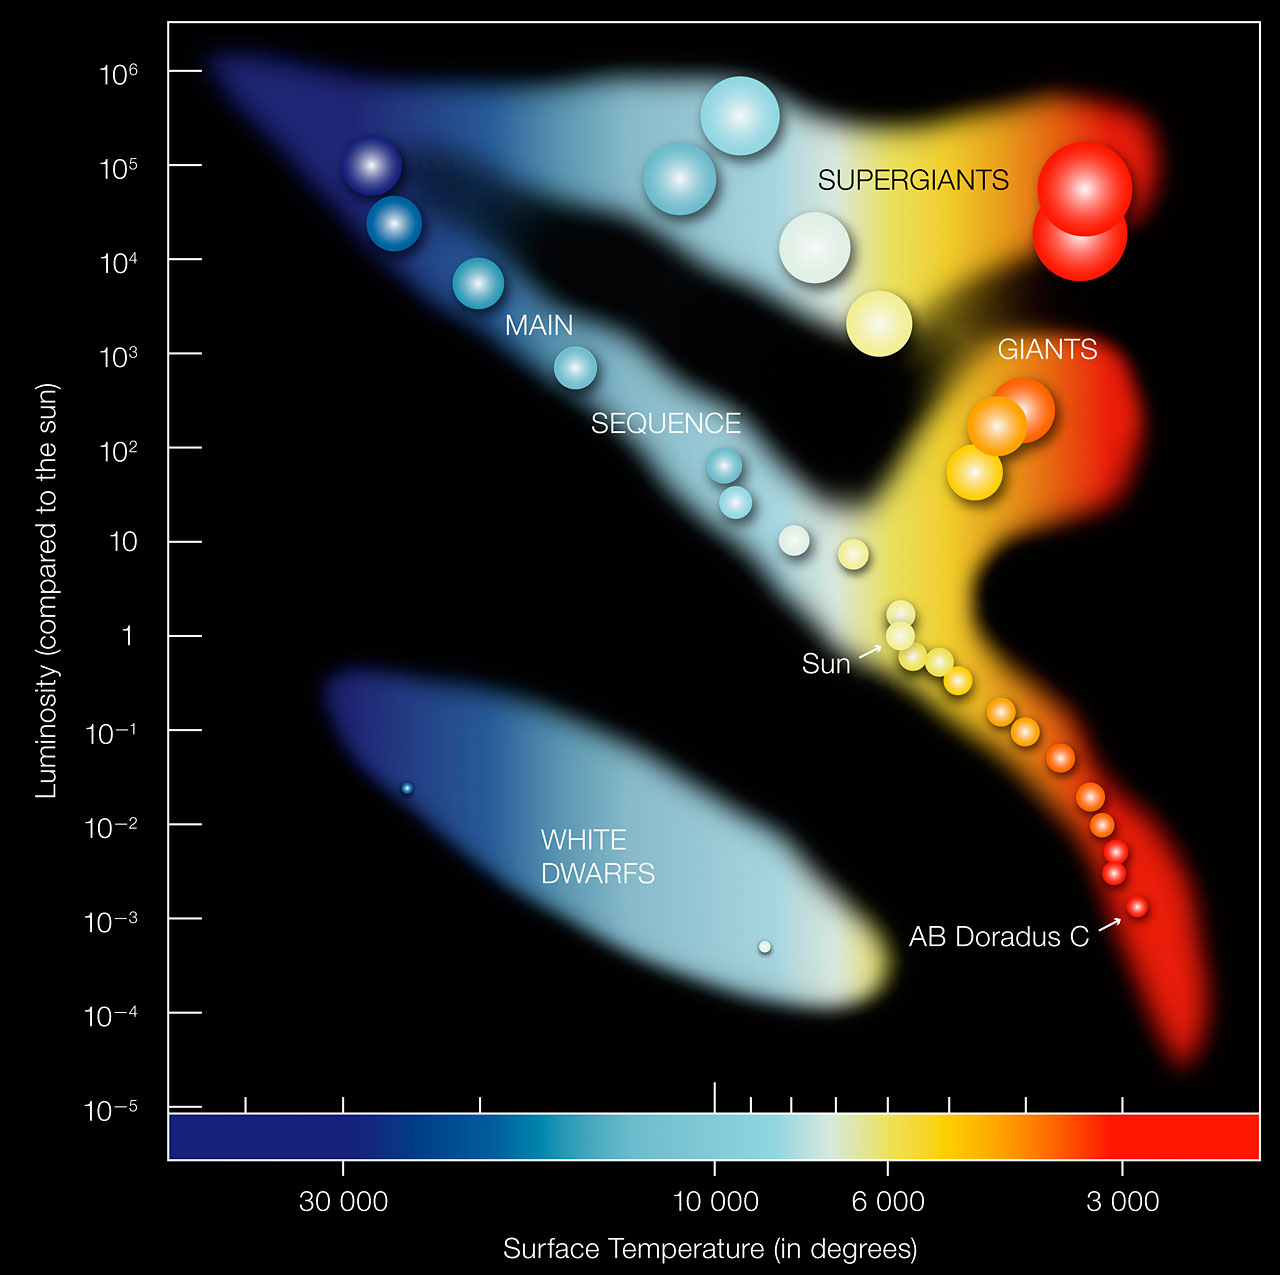
\includegraphics[width=\textwidth]{globular-cluster/eso0728c}
	\caption{Herzsprung-Russell (H-R) diagram, plotting stars according to their luminosity and surface temperature. Luminosity is related to magnitude, and surface temperature is related to color. Image Source: ESO (\url{https://www.eso.org/public/images/eso0728c/}}\label{gc:fig:hr}
\end{figure}

\begin{steps}
	\item Begin to fill out Table~\ref{gc:tab:mag} with the magnitude and distance to a Sun-like star
	in M5. When you finish this lab and turn in this lab report, this table will
	be completely filled out.
\end{steps}

\section{Analyzing the globular clusters near the M87 galaxy}

Figure~\ref{gc:fig:m87} shows the field surrounding the giant Virgo galaxy M87, also known as NGC 4486.

\begin{figure}
	\centering
	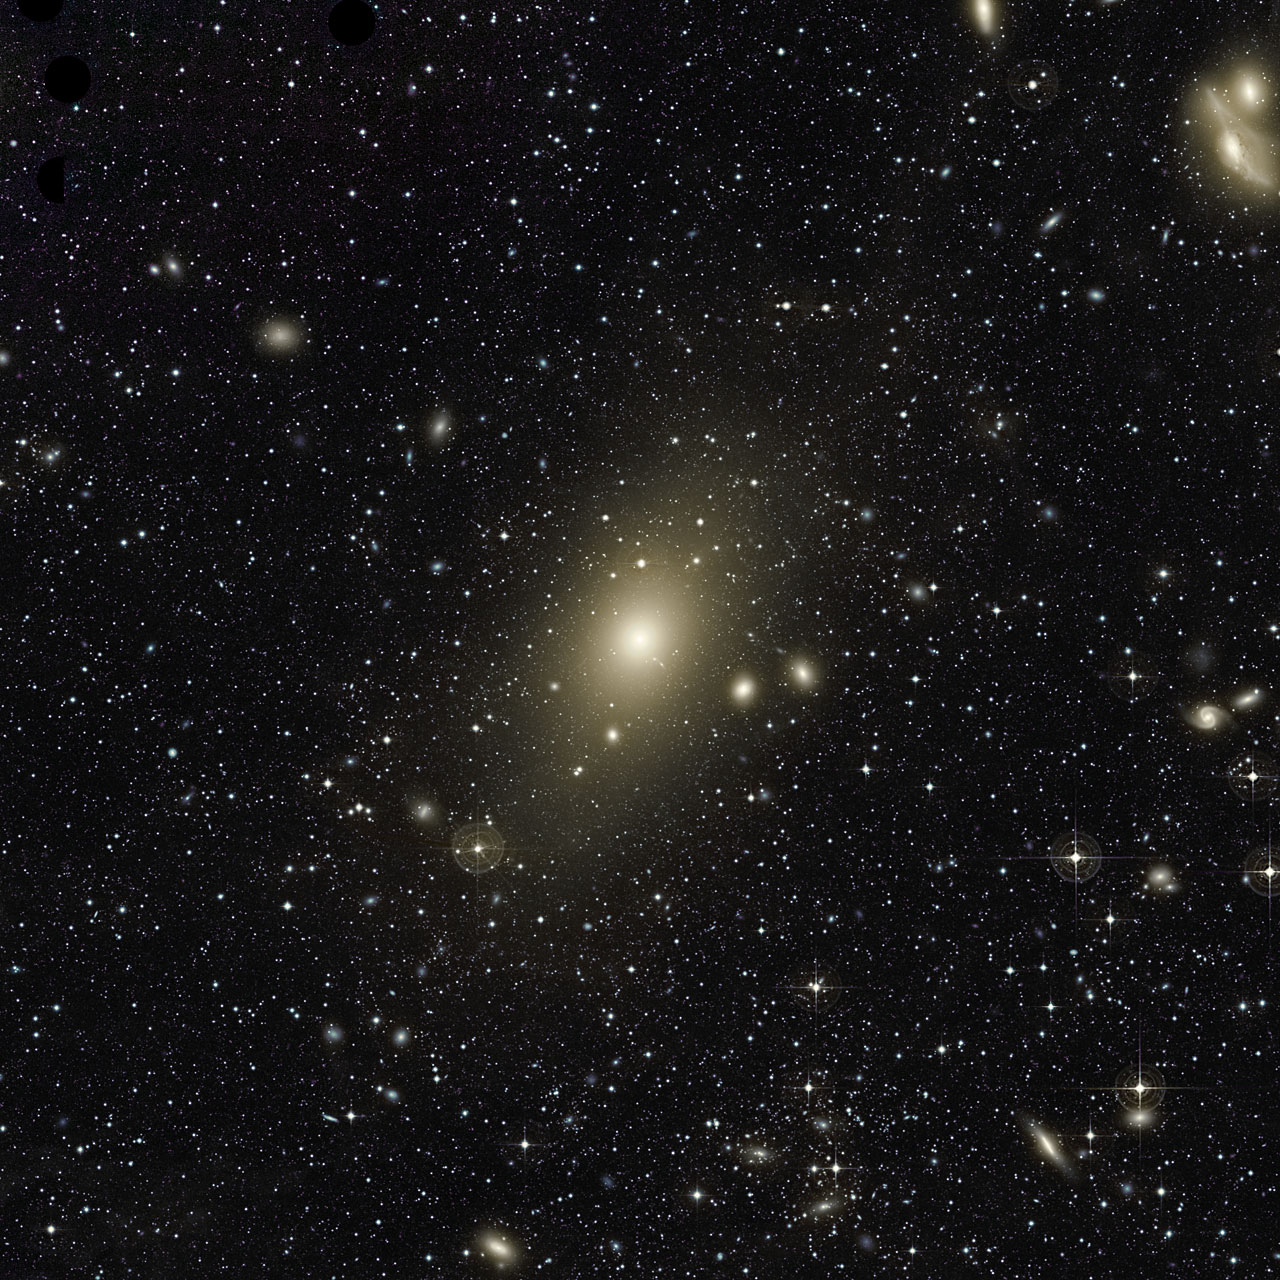
\includegraphics[width=0.7\textwidth]{globular-cluster/eso1525a}
	\caption{Messier 87 (M87) is a nearby elliptical galaxy in the constellation Virgo. It is
		known for having a large population ($\sim 10,000$) of globular clusters, about 100 times more
		than the Milky Way Galaxy. Centered at RA=187.706\textdegree and Dec=12.391\textdegree, the above image
		is 97 arcminutes across. Image source: Chris Mihos (Case Western Reserve University)/ESO, \url{http://www.eso.org/public/images/eso1525a/}.}\label{gc:fig:m87}
\end{figure}

The task is to find the magnitudes for the faint speckles surrounding M87 that are barely visible in
Figure~\ref{gc:fig:m87}, namely its globular clusters. We set up a similar query to that used for M5, except
of course the coordinates (RA, Dec) are different. Enter the following query:

\begin{verbatim}
SELECT TOP 200
   objid,ra,dec,u,g,r, i,z
FROM Star
WHERE
   r BETWEEN 10 AND 23
   AND ra between 187.591 and 187.821
   AND dec between 12.278 and 12.504
\end{verbatim}

The globular clusters are so far away that each cluster of stars appears as, and is categorized as, stars in
the SDSS database. As a cross-check, also run the above query in a random piece of sky at least
5\textdegree away.

\subsection{Questions and results for your report}

\begin{steps}
	\item Make color-magnitude diagrams for both samples (M87 and random-sky)
	and compare them. Does either either color-magnitude diagram show any
	evidence for a correlation between brightness (magnitude) and color for the
	plotted points?
	
	\item Once you have identified which of the sources on your M87 color-magnitude
	diagram can be identified with a population of globular clusters surrounding
	M87, argue which apparent magnitude should be selected to enter into the table, and do so. Why is there a range of magnitudes? How would you make this
	process more precise? What other sources of uncertainty do you think
	there are?
	
	\item Calculate the distance to M87 using Equation~\ref{gc:eq:m-d}, comparing its magnitude to that of M5. If you have not already converted AU to
	parsecs, do so now to get the distance in mega-parsecs ($1\:\mathrm{Mpc} = 2.06 \times
	10^{11}\:\mathrm{AU}$). The accepted value for the distance to the Virgo cluster is 16.4
	Mpc. From your uncertainties above, how well do these two values agree within your expected level
	of uncertainty? See Appendix~\ref{unc:sec:comparing} for details of how to determine this.
	
	\item Based on the distance you found, when did the light from the Virgo galaxy arrive at the sky survey's telescope? What was happening on Earth at that time?
\end{steps}

\section{Include in your report}

Each of the following items will be graded out of 10 points.

\begin{itemize}
	\item Completed table
	
	\item Three color magnitude graphs
	
	\item Questions 1--2 from the first section
	
	\item Questions 3--6 from the second section
	
	\item A 100--200 word reflection on group dynamics and feedback on the lab manual. Address the following topics: who did what in the lab, how did you work together, what successes and challenges in group functioning did you have, and what would you keep and change about the lab write-up?
		
\end{itemize}